\documentclass{article}
\usepackage{amsthm}
\usepackage{amsmath}
\usepackage{graphicx}

\newtheorem{problem}{Problem}

\begin{document}
\title{B-trees}
\author{Henry Z. Lo}
\maketitle

\section{Background}
We first review binary search trees, and show why they are not optimal for storing on disks.  This motivates the need for B-trees.

Though B-trees do not improve on normal trees in terms of $O(n)$, they optimize disk usage.  Thus, they are widely used in databases, and are the basis of the next generation of filesystems.

\subsection{Binary Trees}
Recall how binary search trees (see example in Figure \ref{bst}) organize data:

\begin{figure}
\centering
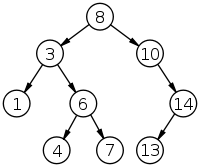
\includegraphics[scale=0.4]{img/bst.png}
\caption{Binary search tree. \label{bst}}
\end{figure}

\begin{itemize}
\item Each node can have at most two children.
\item Left subtree values are less than parent's, and right subtree values are greater.
\end{itemize}

Inserts, removals, and lookups are all done according to these two rules.  With the help of some balancing every now and then, this simple definition allows $O(\log n)$ lookups and inserts.

\subsection{Disk operations}
If all nodes of the tree are stored in random access memory, then operating on a binary search tree is extremely quick.  However, if it is stored on hard disk, then performance is bottlenecked by the disk speed.

In general, any operation involving disk input/output is bottlenecked by disk speed.  This is because read/write requires two physical operations (see for Figure \ref{disk} for terminology):

\begin{itemize}
\item Read/write head must move to the right track (\textit{seek time}, about 4-15 ms).
\item Disk must rotate to put the right sector under the head (\textit{rotational latency}, about 2-6 ms).
\end{itemize}

\begin{figure}
\centering
\includegraphics[scale=0.4]{disk.png}
\caption{Pieces of a hard disk. \label{disk}}
\end{figure}

For a standard 7,200 revolutions-per-minute hard disk, consider the average time for accessing one piece of data (half a revolution):
\begin{align*}
\mbox{average seek time} &= \frac{7200 \mbox{ rotations}}{60 \mbox{ seconds}}\\
 &\approx \frac{1 \mbox{ rotation}}{0.008 \mbox{ seconds}} \\
&= \frac{\mbox{ half rotation}}{0.004 \mbox{ seconds}}
\end{align*}

Compared with CPU operations, which can perform over 10,000 MIPS (million instructions per second), disk I/O is much more expensive:
\begin{align*}
\frac{10000 \mbox{ million instructions}}{1 \mbox{ second}} &= \frac{40 \mbox{ million instructions}}{0.004 \mbox{ seconds}} \\
\end{align*}
Theoretically, in the time it takes to access one piece of data, 40 \textit{million} CPU instructions can be performed.

\subsection{Binary trees for storing data}
As efficient as binary trees are for saving computations, they are not always efficient for storing data on disk.  There are no guarantees for what sectors nodes in a binary tree will be stored.

As an example, let's say you need to store 1024 objects.
\begin{align*}
\mbox{tree depth} &= \log_2 1024 \\
&= 10 \\
\mbox{total seek time} &= \mbox{tree depth} * \mbox{average seek time} \\
&= 40 \mbox{ milliseconds}
\end{align*}

In this same time we can perform 400 million instructions.  

If we stored the objects close together (i.e. in an array), we can cut down on seek time significantly, even if we have to perform $O(n)$ computations.

\section{B-trees}
\subsection{Idea}
One more thing: file systems read and write data in \textit{blocks} (sometimes called clusters), which are groups of sectors.  Filesystems read data block by block.

Every node in a tree is stored in a block.  However, it's a waste of space if the node just contains one key, as they do in binary search trees.  Why not store a bunch of keys in the block, and cut down on the number of disk seeks?  The filesystem will read the whole block anyways.

The idea behind B-trees is to store block-sized nodes.  Each node will contain multiple keys.  Looking in each node will take linear time, but it's much faster than spinning the disc around.

\subsection{Relation to binary trees}
Figure \ref{btree} shows a B-tree.

Note that if a node has $n$ keys, then it has $n+1$ children (unless the node is a leaf).  For example, look at the node with 4 and 7.  It has three children: one with elements less than 4; one with elements between 4 and 7; and one with elements greater than 7.

\begin{figure}
\centering
\includegraphics[scale=0.6]{b-tree.png}
\caption{Example B-tree, which $m=4$. \label{btree}}
\end{figure}

In general, each internal node (not the root or a leaf) can have up to $m$ keys, and $m+1$ children.  Note that when $m=2$, we have a binary search tree.

\subsection{Definition}
Now we are ready to define B-trees.  B-trees have the following properties:
\begin{itemize}
\item Every node except the root must have between $m/2$ and $m$ keys.
\item All leaves are at the same level (this keeps the tree balanced).
\item Non-leaves with $n$ keys have $n+1$ children, as node keys separate node children.
\item Node keys are sorted.
\end{itemize}

Why must nodes have between $m/2$ and $m$ keys?  Well, if they have less than $m/2$, then you can merge two nodes into one block; and if they have more, then they can't fit into one block, so the keys might as well be separated.

\subsection{Implementation}
Now we see how to implement searching/adding/removing in B-trees.

\subsubsection{Searching}
This is the most basic operation.  Because searching does not alter the contents of the B-tree, we don't need to do anything to keep the tree within the definition.  The following procedure will search for an object $x$:

\begin{enumerate}
\item Start at the root.
\item Find the key $k_i$ such that:
\begin{itemize}
\item $x < k_i$ and $k_i$ is the first key (i.e. $i=1$), OR
\item $k_i < x < k_{i+1}$, OR
\item $k_i < x$ and $k_i$ is the last key (i.e. $i=m$)
\end{itemize}
\item Travel to the $i^{th}$ child.
\item Continue step 2 until we get the leaf.
\item Look for $x$ in the leaf.
\end{enumerate}

We can perform step 2 using binary search in $O(\log m)$ time.  This does \textit{not} depend on the number of elements being stored, as $m$ is a user-selected parameter.

Travelling to the $i^{th}$ child will take $O(\log n)$ time, where $n$ is the number of elements.  We don't need to consider $m$ as it doesn't change, so searching takes $O(\log n)$ time.

\subsubsection{Insertion}
We can insert $x$ using the same procedure as searching.  However, if the leaf we end up in is full, then we need to split the node.  We can do this in the following way (see Figure \ref{btree-insert} for a visual):

\begin{figure}
\centering
\includegraphics[scale=0.6]{b-tree-insert.png}
\caption{Insertion in a B-tree with $m=2$. \label{btree-insert}}
\end{figure}

\begin{enumerate}
\item In the current leaf, take the median and insert it into the parent.
\item Take everything in the current node which is less than the median and put it into one child of the parent.
\item Take everything greater than the median and put it into another child of the parent.
\end{enumerate}

If the parent overflows, then we perform the same procedure on the parent. If the root overflows, then we grow the tree by one level.

This happens in Figure \ref{btree-insert} when we insert 7.  The insertion causes the rightmost leaf to overflow, sending 6 to its parent; that causes the parent to overflow, sending 4 to a new root.

Steps 1-3 can all be done in constant time (this is binary search), though copying data to new nodes is $O(m)$.  In the worst case, we have to split nodes from leaf to root - this is $O(\log n)$.  Taking into account the $O(\log n)$ lead insert, the whole insertion procedure is $O(\log n)$.

\subsubsection{Removal}
When removing an element causes the leaf to have less than $m/2$ elements, the leaf must be rebalanced.  This is done by either stealing a key from a sibling, or merging with a sibling.

For stealing a key:
\begin{enumerate}
\item Take the sibling's largest key (if left sibling), or smallest key (if right sibling).
\item Insert key into parent, replacing the key for the current leaf.
\item Put the replaced key in the leaf.
\end{enumerate}

When both siblings are the minimum size, we pick one sibling and merge:
\begin{enumerate}
\item Suppose we merge left.  Then we take the left node's separator and put it in the leaf.
\item Move everything in current leaf to left leaf.
\item Parent now loses an element, and may need rebalancing.
\end{enumerate}

Both procedures only depend on $m$, though merging may cause the rebalancing to propagate to the root (occurring $O(\log n)$ times.)

\section{Indexing}
\subsection{Hashing vs. B-trees}
Despite their speed advantages, B-trees are used as indexes in databases more often than hashing.  Hashing doesn't support range queries, and so have limited applicability.  Ordering allows B-trees to do the following:

\begin{itemize}
\item Search based on prefixes, e.g. find all keys that begin with "Pat".
\item Range queries, e.g. find all keys less than 10.
\end{itemize}

In addition, B-trees are auto-balanced, and avoid the expensive $O(n)$ rehashing that hash tables require every now and then.  The comparisons between trees and hashing discussed in previous lectures also hold.

\subsection{B+ trees}
In practice, B+ trees are used in databases and filesystems (e.g. MySQL, NTFS, SQL server, ReiserFS).  B+ trees differ in two important ways (see Figure \ref{bplus} for an example):

\begin{figure}
\centering
\includegraphics{bplus.png}
\caption{B-plus tree example. \label{bplus}}
\end{figure}

\begin{itemize}
\item Leaves have pointers to their right sibling leaves.
\item Only key information is stored in nodes; all data are children of leaves.
\end{itemize}

Both of these points help facilitate range queries.  Note that in a standard B-tree (and in a binary tree), getting a range of values requires traversing up and down the tree.  In a B+ tree, we can simply find the first value in the range, then follow it until we get the number of elements that we want; this is simpler and faster.

The rules for B+ trees also have the following effects on the tree structure:

\begin{itemize}
\item Leaves having a pointer to other leaves means that their maximum capacity is decreased by one.
\item A parent's keys are replicated among its children.
\item This leads to more nodes in general.
\item B+ trees take up slightly more memory as a result.
\end{itemize}

\end{document}
